\section{Introduzione}
Il progetto ha lo scopo di fornire un servizio online di aste per la compravendita di oggetti, basato su blockchain. Sotto il controllo di un manager, ogni utente può creare un'asta o interagire con un'asta già attiva. Esistono due tipi di aste, l'asta inglese e l'asta vicrey. Il manager non può prendere parte a nessuna delle aste attive, mentre un venditore non può prendere parte alla propria asta, tutto ciò per evitare che il processo d'asta sia corrotto. Inoltre alla fine di ogni asta, il trasferimento dell'ammontare dovuto viene bloccato all'interno del contratto associato all'asta, solo il vincitore può sbloccare tale trasferimento, a meno che non siano passati 5 giorni (nello specifico 1440 blocchi) dalla conclusione dell'asta in oggetto. In questo modo si vuole evitare che il venditore o il vincitore si tirino indietro nel momento del pagamento o della spedizione del bene.
\section{Scelte di progettazione}
Nel progetto sono presenti tre smart contract scritti in \textit{Solidity}: \texttt{EnglishAuction} (\textbf{EA}), \texttt{VicreyAuction} (\textbf{VA}) e \texttt{AuctionManager} (\textbf{AM}).
Gli indirizzi delle aste create tramite l'AM vengono salvati all'interno di esso, in modo che sia possibile raggiungere tali aste tramite l'AM stesso. Inoltre il manager del servizio ha la possibilità di bloccare la creazione delle aste (ed eventualmente sbloccarla), sia per distruggere l'AM quando tutte le aste già attive siano concluse, sia per evitare che il numero di aste attive cresca in modo incontrollabile. Di seguito sono riportate delle brevi descrizioni dei metodi definiti all'interno dell'AM:
\begin{itemize}
	\item \texttt{createEnglishAuction(...)}: se \texttt{couldCreateAuction == true}, crea una nuova istanza di un contratto EA, chiamando il suo costruttore e salvandone l'indirizzo;
	\item \texttt{createVicreyAuction(...)}: se \texttt{couldCreateAuction == true}, crea una nuova istanza di un contratto VA, chiamando il suo costruttore e salvandone l'indirizzo;
	\item \texttt{deleteEnglishAuction(...)}: rimuove un indirizzo dalle aste EA salvate, viene chiamata direttamente dal contratto dell'asta da eliminare quando essa viene conclusa;
	\item \texttt{deleteVicreyAuction(...)}: rimuove un indirizzo dalle aste VA salvate,  viene chiamata direttamente dal contratto dell'asta da eliminare quando essa viene conclusa;
	\item \texttt{getEnglishAuctions()}: restituisce tutti gli indirizzi delle aste EA attualmente attive;
	\item \texttt{getVicreyAuctions()}: restituisce tutti gli indirizzi delle aste VA attualmente attive;
	\item \texttt{stopCreation()}: se \texttt{couldCreateAuction == true}, lo pone a \texttt{false};
	\item \texttt{startCreation()}: se \texttt{couldCreateAuction == false}, lo pone a \texttt{true};
	\item \texttt{destroyManager()}: se non vi sono aste attive, chiama il metodo \texttt{selfDestruct}.
\end{itemize}
\begin{figure}[h]
	\centering
	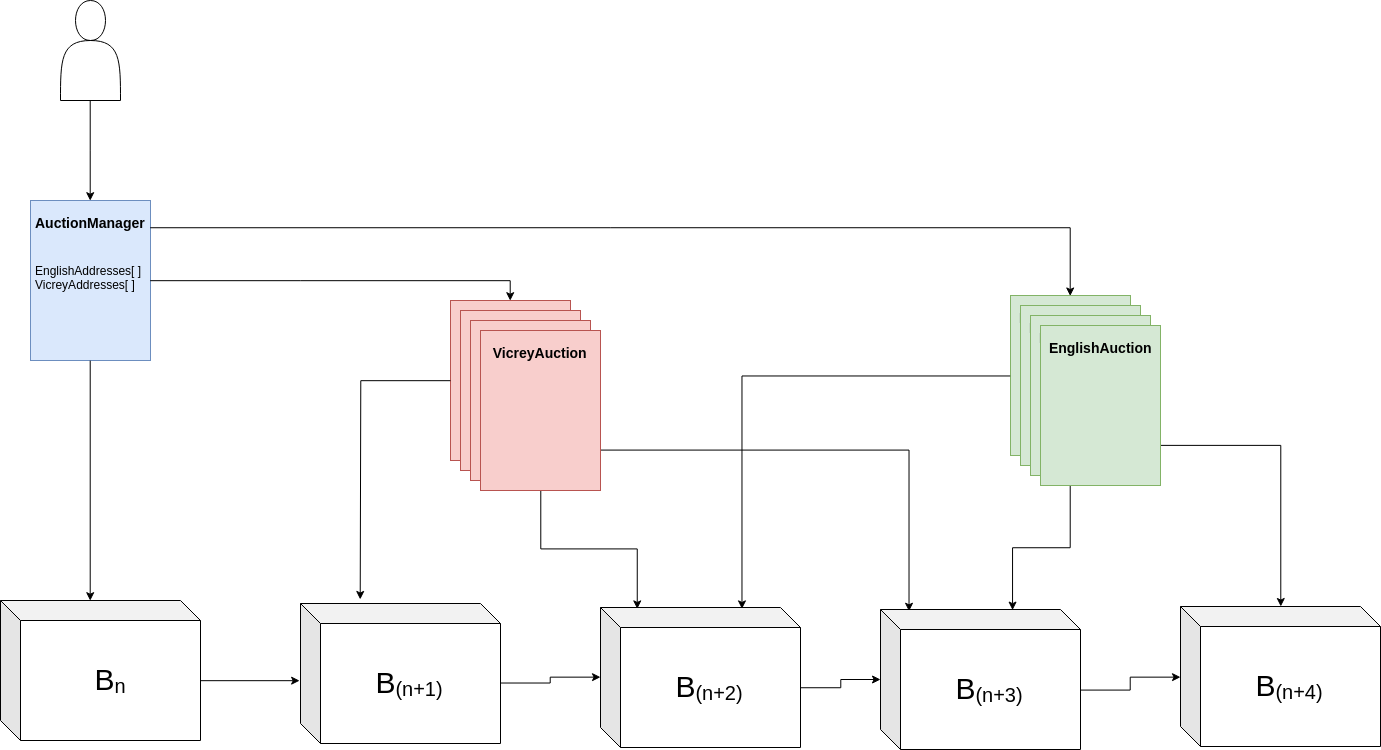
\includegraphics[scale=0.3]{contratti.png}
	\caption{Diagramma della struttura dei contratti.}\label{fig1.1}
\end{figure}
Grazie a questo sistema, per fornire il servizio di aste è necessario condividere solo l'indirizzo dell'AM e non tutti gli indirizzi delle aste. Inoltre tramite l'indirizzo del manager (colui il quale ha generato l'AM) è possibile gestire le fasi delle aste attive. Le fasi delle aste sono infatti scandite dal passare dei blocchi all'interno della blockchain, ogni 5 blocchi è possibile passare alla fase successiva. Potrebbe però accadere che un venditore, ad esempio in una EA, non abbia ricevuto alcuna offerta alla fine della fase di puntata, in tal caso il venditore non è più interessato a finalizzare l'asta ed eliminarla dalla blockchain e dall'AM. Per questo motivo il manager ha la possibilità di cambiare fase ad un'asta in ogni momento (basta che siano ovviamente passi i 5 blocchi di default per la durata di una fase).  Lo stesso discorso può essere fatto se una qualsiasi asta fosse bloccata nella fase di finalizzazione, in tal caso il manager può finalizzare egli stesso l'asta se e solo se siano tale fase sia bloccata da circa 5 giorni (1440 blocchi).\newline
Infine si è deciso di utilizzare un server MySql per salvare "Titolo" e "Descrizione" delle varie aste. Utilizzare direttamente i contratti per salvare stringhe di grande dimensioni è costoso in quanto l'utilizzo efficiente e minimale della memoria all'interno della blockchain è una proprietà fondamentale per lo sviluppo di un buon SmartContract, infatti l'operazione associata allo \texttt{STORAGE} di variabili in memoria è la più costosa. Da un punto di vista della sicurezza, questa decisione non implica nessuna minaccia in quanto "attaccare" il database per modificarne le informazioni salvate al suo interno, non produrrebbe alcun effetto sulla blockchain e potrebbe essere facilmente individuato e corretto.
\section{Scelte implementative}
\subsection{Contratto AuctionManager}
Nel contratto AM gli indirizzi delle aste attive sono salvati tramite l'utilizzo di un \texttt{mapping} (usando come chiavi l'indirizzo del contratto) e di un \texttt{array} di supporto. La prima struttura viene utilizzata per controllare l'esistenza di un dato indirizzo all'interno di quelli attivi, in modo da avere un accesso a costo unitario. L'\texttt{array} viene invece utilizzato laddove è necessario usare l'indirizzo stesso del contratto, infatti in \texttt{Solidity} non è possibile accedere alle chiavi di un \texttt{mapping} ma solo al loro valore. Visto questo tipo di struttura, quando occorre eliminare un'asta dal contratto AM è necessario spostare l'ultimo elemento dell'\texttt{array} nella posizione lasciata vuota dall'elemento eliminato e , soprattutto, bisogna diminuire la lunghezza dell'\texttt{array}. Gli \texttt{array} dinamici, infatti, mantengono la proprio dimensione anche dopo aver chiamata la funzione \texttt{delete} sul l'elemento specificato, portando a comportamenti indesiderati soprattutto nel caso in cui si vogliano accedere gli elementi nelle utlime posizioni.\newline
\subsection{Contratti EnglishAuction e VicreyAuction}
Il passaggio di fase viene eseguito tramite l'utilizzo di un \texttt{modifier}. Prima dell'esecuzionedel codice associato alla transazione, viene controllato se siano passati 5 blocchi dall'ultimo cambiamento di fase, in caso affermativo la fase viene avanzata. Il controllo della fase viene quindi fatto tramite un secondo \texttt{modifier} che confronta la fase attuale con la fase associata alla transazione. In questo modo è possibile eseguire una transazione anche se questa è associata alla fase successiva a quella attuale, in quanto essa viene modificata direttamente dalla transazione eseguita.
\subsection{DAPP}
Per lo sviluppo della DAPP, sono stati necessari diversi FrameWork e libreria per impostare tutto l'environment necessario per testare e implementare sia i contratti che la DAPP stessa. Per la precisione si è fatto uso di:\newline
\begin{itemize}
 	\item \textbf{Truffle}: un FrameWork necessario a testare e deployare i contratti;
 	\item \textbf{Web3}: una libreria necessaria per interagire tramite javascript con i contratti sulla blockchain;
 	\item \textbf{Truffle-contracts}: una libreria simile a Web3, con qualche funzionalità in meno, rende l'interazione con i contratti più semplice ed intuitiva;
 	\item \textbf{NodeJS}: un FrameWork utilizzato per gestire la DAPP sviluppata in javascript e jquery, e per interagire con Truffle;
 	\item \textbf{lite-server}: una libreria utilizzata come server per "servire" la DAPP e i suoi moduli;
 	\item \textbf{bn.js}: una libreria in javascript necessaria a manipolare i valori dei numeri utilizzati dai contratti della blockchain (e.g. uint256, o valori in Wei), evitando errori di integer overflow e di precisione;
 	\item \textbf{MetaMask}: un'estensione del browser che permette di collegarsi ai nodi della blockchain, in modo da poter interagire con diverse blockchain sia di testi che reali;
 	\item \textbf{Ganache}: una blockchain locale di testing, permette di simulare una vera rete su cui è possibile deployare e conseguentemente interagire con i contratti scritti in Solidity;
 	\item \textbf{Boostrap}: una serie di librerie di stile CSS e javascript per renderizzare la DAPP;
 	\item \textbf{Express} : una libreria javascript server-side per salvare i dati delle aste quali "titolo" e "descrizione" in un server MySql;
 	\item \textbf{Truffle-assertion} : una libreria di NodeJS per testare i contratti;
 	\item \textbf{Truffle-assertion} : un nodo che permette di interfacciarsi alle varie blockchain online.
\end{itemize}
\begin{figure}[h]
	\centering
	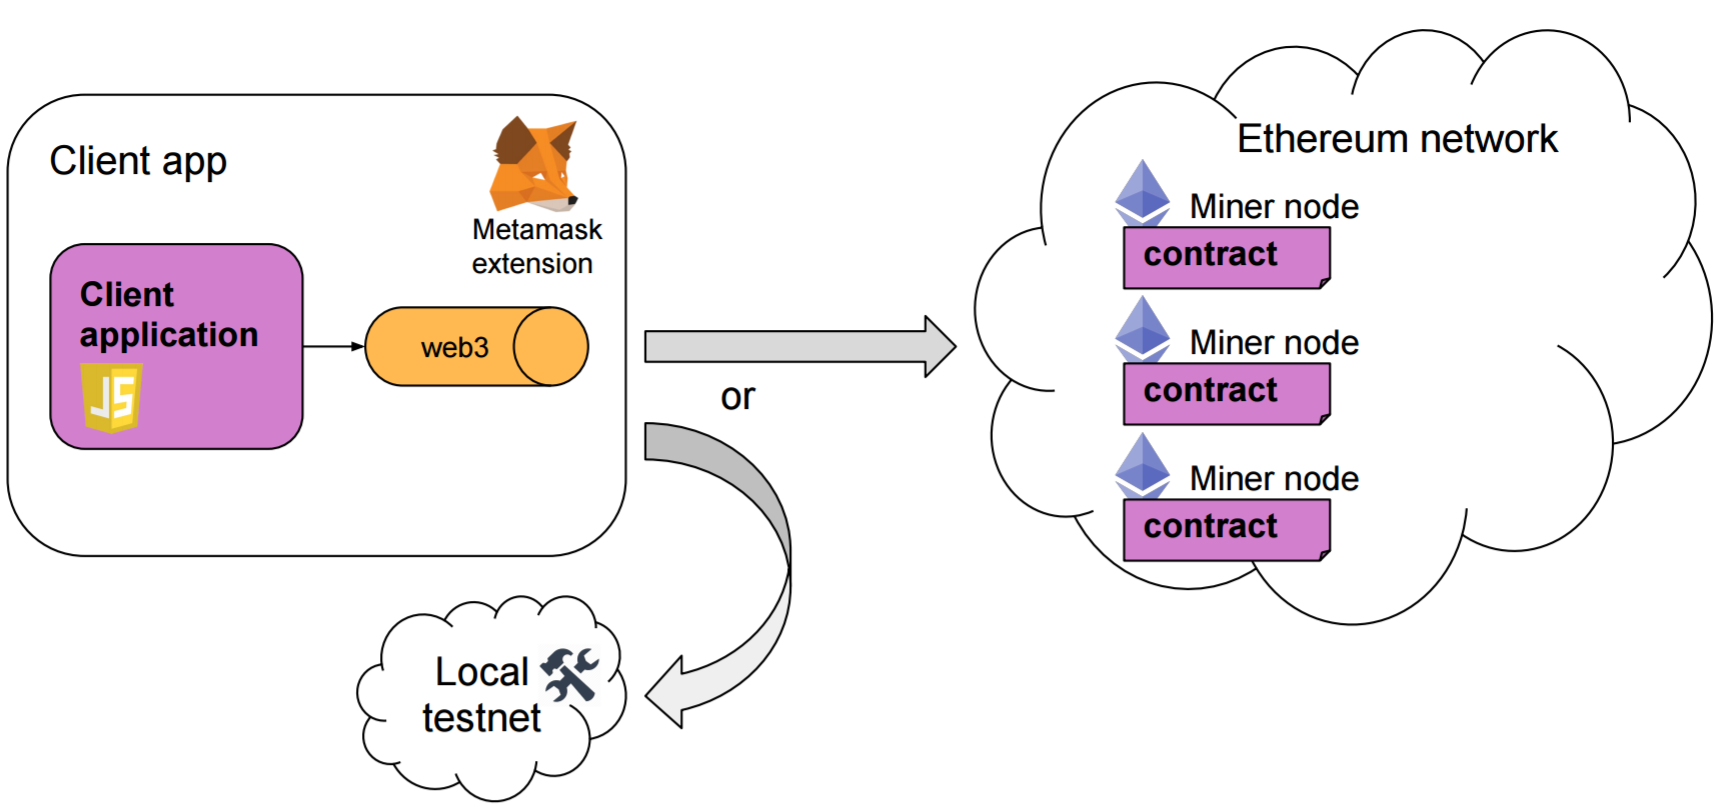
\includegraphics[scale=0.3]{suite.png}
	\caption{Environment parziale per interfacciarsi al mondo delle blockchain.}\label{fig1.2}
\end{figure}
L'interfaccia della DAPP è dinamica, si adatta infatti all'account attivo in MetaMask. Se tale account corrisponde al creatore dell'AM, verranno mostrate le aste in cui la fase è sospesa da 576 blocchi (circa 2 giorni), quelle in fase di \texttt{Pending} e quelle nella fase di \texttt{Finalizing} (cioè quelle aste con cui il manager può interagire), divise per tipo. Inoltre, nella parte superiore dell'interfaccia è presente un pannello che permette di gestire tutto il servizio offerto. Sono mostrati il numero di aste attive e sono presenti dei pulsanti che permettono di bloccare/sbloccare la creazione di aste e di distruggere l'AM.
Se, invece, l'account attivo in MetaMask non è quello del manager, l'interfaccia si presenta divisa in tre sezione, una per tipologia di contratto più una sezione in cui è possibile creare una nuova asta. Non tutte le aste attive saranno mostrate all'utente, nell'interfaccia le aste sono infatti divise in 3 categorie:
\begin{itemize}
	\item \textbf{Owned Auctions}: tutte le aste attive di cui l'account attivo è proprietario;
	\item \textbf{Open Auctions}: tutte le aste attive con cui un nuovo utente può interagire, quindi faranno parte di questa categoria tutte le aste in fase di apertura (e.g. \texttt{Glory Phase} o \texttt{Commitment})  e tutte quelle aste in cui l'utente è presente nel caso specifico delle VA (e.g. \texttt{Withdrawal} o \texttt{Opening} se l'utente ha eseguito un'offerta) ;
	\item \textbf{Closing Auctions}: tutte le aste attive in \texttt{Finilizing Phase} e \texttt{Pending Phase}  di cui l'account attivo è vincitore.
\end{itemize}
A seconda della fase in cui si trova ogni asta, verranno mostrate le informazioni necessarie all'utente e dei pulsanti che permettono di interagire con essa tramite le varie transazioni del contratto (e.g. tutte le transazioni "legali" all'interno della fase attuale dell'asta). Sono inoltre presenti due pulsanti per ogni asta, uno permette di aggiornare le informazioni associate alla stessa, in modo da poter tenere sotto controllo lo sviluppo dell'asta. Il secondo pulsante permette invece di ascoltare gli eventi emessi sulla blockchain dal contratto associato all'asta. Per evitare di sovraccaricare la DAPP e il nodo con cui essa si interfaccia alla blockchain, non è possibile eseguire più di 20 sottoscrizioni per volta. Inoltre se si esegue il refresh della pagina direttamente dalla barra degli indirizzi, si perdono tutte quante le sottoscrizioni e anche lo stato delle varie transazioni in esecuzione.\newline
Infatti dopo aver attivato un pulsante associato ad una transazione, viene creata una \texttt{Promise} che eseguirà la transazione tramite MetaMask e ritornerà il risultato associato ad essa solo dopo che la transazione viene eseguita sulla blockchain. In questo intervallo di tempo, vengono disabilitati i pulsanti associati alla transazione e al refresh della singola asta, in modo da evitare di eseguire più volte la stessa transazione.\newline
Infine in entrambe le interfacce vi è la sottoscrizione all'evento di creazione di una nuova asta, in modo da aggiornare e tenere sempre informato l'utente sullo stato del servizio. In questo modo non è necessario eseguire il refresh della pagina per dover ricaricare tutte le nuove aste createsi durante l'utilizzo della DAPP.
\begin{figure}[h]
	\centering
	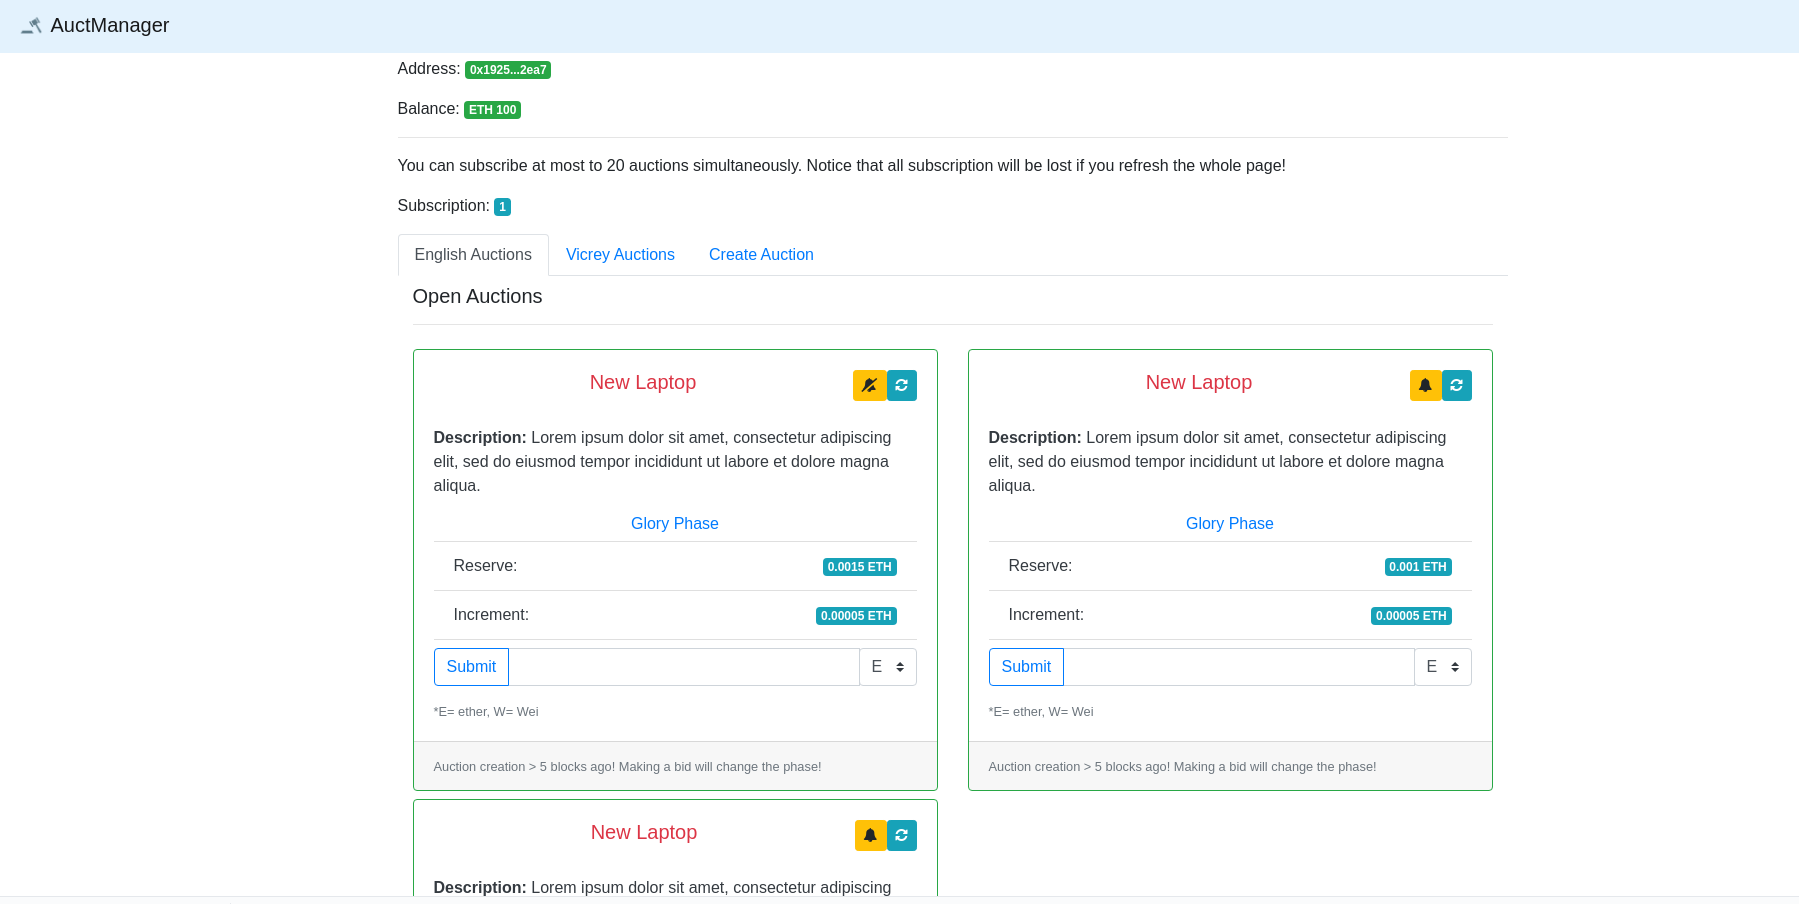
\includegraphics[scale=0.3]{interface.png}
	\caption{DAPP interface.}\label{fig1.3}
\end{figure}
\section{Testing}
\subsection{Test Contratti}
Per testare i contratti sono stati scritti dei test specifici con Truffle in cui vengono testate alcune situazioni particolari. Per le EA vengono eseguiti 4 test specifici:
\begin{itemize}
	\item "Test \_Buy Out the good": si eseguono una serie di transazioni per comprare il bene prima che cominci l'asta;
	\item "Test \_Same address 2 bids \_A lower bid!": prima si cerca di fare due puntate dallo stesso account, poi si cerca di fare una puntata più bassa di quella attualmente vincente;
	\item "Test \_No bids": si crea e conclude l'asta senza fare alcuna puntata;
	\item "Test \_Revert: out right phase, can interact, can finilize, can pending": si eseguono una serie di transazioni per testare le condizioni di revert del contratto.
\end{itemize}
Per le VA sono stati scritti i seguenti test:
\begin{itemize}
	\item "Test \_Same bid, withdraw": si esegue un withdraw e si controlla che non sia possibile eseguire due puntate dallo stesso account;
	\item "Test \_Low commitment, No bids": si esegue una puntata inferiore al prezzo di riserva, dopo di che si conclude l'asta senza altre puntate;
	\item "Test \_3 different bid, the second lower than the third!": si eseguono una serie di transazioni per arrivare alla fase di opening e controllare che se la seconda puntata è più bassa sia della prima che della terza (in ordin edi apertura) anche il prezzo del bene venga aggiornato (pari alla seconda puntata più alta);
	\item "Test \_Revert: out right phase, no deposit, can interact, can finilize, can pending, no in auction open and withdraw": si eseguono una serie di transazioni per testare le condizioni di revert del contratto.
\end{itemize}
Per l'AM sono stati implementati i seguenti test:
\begin{itemize}
		\item "Test \_Stop and enable creation from manager auction": si testa lo stop e l'avvio della creazione delle aste;
	\item "Test \_Create 3 english auctions, delete the first and check the order": si controlla come evolve l'ordine delle aste EA all'interno dell'array eliminando un'asta in posizione centrale;
	\item "Test \_Create 3 vicrey auctions, delete the first and check the order":stesso test precedente ma per le aste VA;
	\item "Test \_Call function from wrong addresses, destroy the manager contract with active auctions": si eseguono una serie di transazioni per testare le condizioni di revert del contratto.
\end{itemize}
Per eseguire tali test è stato utilizzato Ganache con la funzione di "automining" attiva, la fase è stata controllata e fatta avanzare tramite un ciclo while richiamando la fase del contratto. I test infatti risultano essere lenti, in particolare è necessario impostare l'automining pari a 5 secondi per non incorrere in errori. Per eseguire i test occorre anche eseguire il server express dopo aver lanciato l'esecuzione del server MySql, in particolare è necessario che esso contenga un DB di nome "AuctionList" contente due differenti tabelle "english" e "vicrey", le varie informazione per la connessione sono presenti nel file "server/server.js" e "server/model/db.js". Dopo di che basterà eseguire i diversi test, di seguito sono mostrati i vari comandi da eseguire in terminali diversi:
\begin{verbatim}
1: $ ganache-cli -p 8545 -b 5
\end{verbatim}
\begin{verbatim}
2: $ node server/server.js
\end{verbatim}
\begin{verbatim}
3: $ truffle test 
\end{verbatim}
\subsection{Test DAPP}
Per eseguire un test sul funzionamento della DAPP occore installare MetaMask nel browser e lanciare sia lite-server (port:3000) che express (port:5000). Dall'icona di MetaMask è possibile selezionare la network di testing (port:8545) che viene emulata ancora una volta con Ganache. Per far si che MetaMask si connetta ad un account della block chain, è necessario copiare uno degli indirizzi che Ganache mette a disposizione (il numero 3 è stato utilizzato come predefinito) e copiare l'Api key all'interno di MetaMask. Inoltre, è necessario deployare i contratti, a tal proposito, nel file \texttt{truffle-config.json} sono state definite due network. La prima è quella utilizzata per i test su Ganache, la seconda viene utilizza per la connessione alla block chain di test di Ropsten. Per deployare il contratto manager in locale e eseguire la Dapp, è necessario eseguire i seguenti comandi in terminali diversi:
\begin{verbatim}
1: $ ganache-cli -p 8545 -b 5
\end{verbatim}
\begin{verbatim}
2: $ node server/server.js
\end{verbatim}
\begin{verbatim}
3: $ truffle migrate --reset --network  development
3: $ npm run dev
\end{verbatim}
Il flag "network" indica su quale rete verrà eseguito il file di "migrazione" dei contratti. Nel file \texttt{2\_deploy\_contracts.js} sono definiti i vari comandi per deployare i diversi contratti a seconda della rete in cui ci si trova. Quindi connettendosi a Ganache verranno istanziati diversi contratti per popolare appropriatamente la DAPP durante il test. In particolare si consiglia di configurare MetaMask con l'account numero 3, o con il numero 0 se si vuole vedere l'interfaccia dal punto di vista del manager. Non essendo necessario un login per diversificare gli account, occorre settarli manualmente all'interno di MetaMask.
\subsection{Test Ropsten}
Infine il progetto è stato testato anche sulla rete pubblica Ropsten, utilizzando come nodo di accesso Infura (la secre key non sarà inclusa nel progetto). Basterà eseguire lo stesso comando visto in precedenza con la giusta network. In ogni contratto è raggiungibile un metodo di \texttt{selfdestruct} per evitare di lasciare contratti svincolati sulla network pubblica. Nel file \texttt{2\_deploy\_contracts.js} se la network riscontrata è quella di Ropsten, verrà deployato solo ed esclusivamente l'AM. Per eseguire i test su tale rete, basta creare alcuni account direttamente da MetaMask che fornisce 3ETH da spendere nella testnet. Bisognerà quindi eseguire i seguenti comandi in terminali diversi:
\begin{verbatim}
1: $ node server/server.js
\end{verbatim}
\begin{verbatim}
2: $ truffle migrate --reset --network  ropsten
2: $ npm run dev
\end{verbatim}
A differenza dei test eseguiti in locale, le transazioni sulla testnet sono più lente, in quanto i blocchi vengono "minati" realmente ed occorre quindi attendere tali tempi di attesa.
\section{Conclusioni e eventuali lavori futuri}
Una cosa da notare è come sia la libreria Web3 che MetaMask eseguono la stima della quantità necessaria di gas per ogni transazione. Ogni transazione infatti ha un quantitativo di gas limite che l'utente è disposto a spendere per eseguire una data transazione. Se tale esecuzione comporta una spesa superiore al limite impostato, l'esecuzione termina e tutto il gas viene consumato. La stima fatta però tiene conto anche del gas che viene reso per via di alcune operazione che, invece di "costare" gas, lo restituiscono, ad esempio il riportare una variabile al suo valore di default (e.g. address = 0x0). Quindi se ad esempio una transazione ha costo 2000 gas e restituisce 500 gas, la stima fatta (ed impostata come gas limite da MetaMask di default) sarà pari a 1500 gas. Questa stima però nasconde un problema, il gas restituito viene reso solo DOPO l'esecuzione della transazione, ciò significa che se come gas limite si pone 1500 gas, la transazione fallirà. comportando la perdita totale dell'ammontare indicato. Per evitare tali casistiche, nelle transazione in cui sono presenti delle operazioni che restituiscono gas, si è prima eseguita una stima del gas necessario con Web3, dopo di che si esegue la transazione imponendo come gas limite il doppio del valore stimato. Si è impostato il doppio in quanto , come riportato dal "Yellow Paper" il gas restituito ha un tetto massimo pari alla metà del costo della transazione. Ciò significa che se una transazione costa 2000 gas e il gas restituito è pari a 1500 gas, la transazione costerà in totale 1000 gas e non 500 gas. Perciò, al massimo l'effettivo costo di una transazione sarà pari al doppio della sua stima. Tale regola è necessaria per evitare che i minatori non guadagnino nulla dalla convalida di una transazione o addirittura siano portati a dover "pagare" per "minare" una transazione all'interno di un blocco.\newline
Ciò che manca all'interno della DAPP è sicuramente il tenere traccia delle transazione in "pending", cioè in esecuzione. Si è infatti voluto evitare di utilizzare tecnologie come i cookie per salvare lo stato di tale transazioni, per non incorrere in problemi di sicurezza. Tale stato però si potrebbe comunque ricercare all'interno della blockchain stessa conoscendo l'indirizzo dell'asta a cui si è interessato. 
Inoltre, all'interno dei contratti non è considerata la casistica in cui al vincitore debba essere restituito lì'importo della propria puntata nel caso in cui ad esempio il venditore non si prenda carico della spedizione del bene.
infine, impostando il prezzo per unità di gas pari a 20 GWei, la creazione di un'asta (nel particolare la creazione della prima asta avrà un costo maggiore, come tutte quelle operazioni che inizializzano il valore di una variabile settata ancora al valore di default) viene a costare all'utente circa 0.50 cent di euro, un costo molto contenuto rispetto al profitto che esso può avere dalla vendita di un bene ed essendo tale operazione la più costosa che un venditore si troverà a fronteggiare.